\usepackage[english] {babel}
\usepackage[T1]      {fontenc}

\usepackage{amsmath, amsfonts, graphicx}
\usepackage{bibunits, tikz}

\usetheme{progressbar}

\setbeamersize
  {text margin left=1em, text margin right=1em}

\title
  [Short Title]
  {Full Title of the Presentation}

\author
  [Bruce Wayne]
  {Bruce Wayne\quad Clark Kent\\Peter Parker\quad Alan Scot}

\date
  {April 01, 2011}

\institute
  {Justice League of America}

\begin{document}

\maketitle

\begin{frame}{Overview}

  \tableofcontents

\end{frame}

\section
  {Introduction}

\begin{frame}
  {Introduction}

  Things in a Bulleted List\pause

  \begin{enumerate}
  \item Bullets that
    \begin{enumerate}
    \item one
    \item two
    \end{enumerate}\pause
  \item Come up
    \begin{enumerate}
    \item one
    \item \emph{two} and three
    \end{enumerate}\pause
  \item One by one
    \begin{enumerate}
    \item one
    \item two
    \end{enumerate}
  \end{enumerate}
\end{frame}


\section
  {Main Body}

\subsection{Equations}

\begin{frame}
  {Equations}

  Equations are easy
  \begin{itemize}
  \item Just copy/paste equations\pause
  \item From the paper!
    \begin{equation*}
      \textbf{p}^* = \underset{\textbf{p}}{\arg\!\min}~\sum_{\textbf{x}}\left[ I(\textbf{W}(\textbf{x};\textbf{p})) - T(\textbf{x}) \right]^2
    \end{equation*}
  \end{itemize}
\end{frame}


\begin{frame}
  {Pictures}

  \begin{figure}[t]
    \centering
    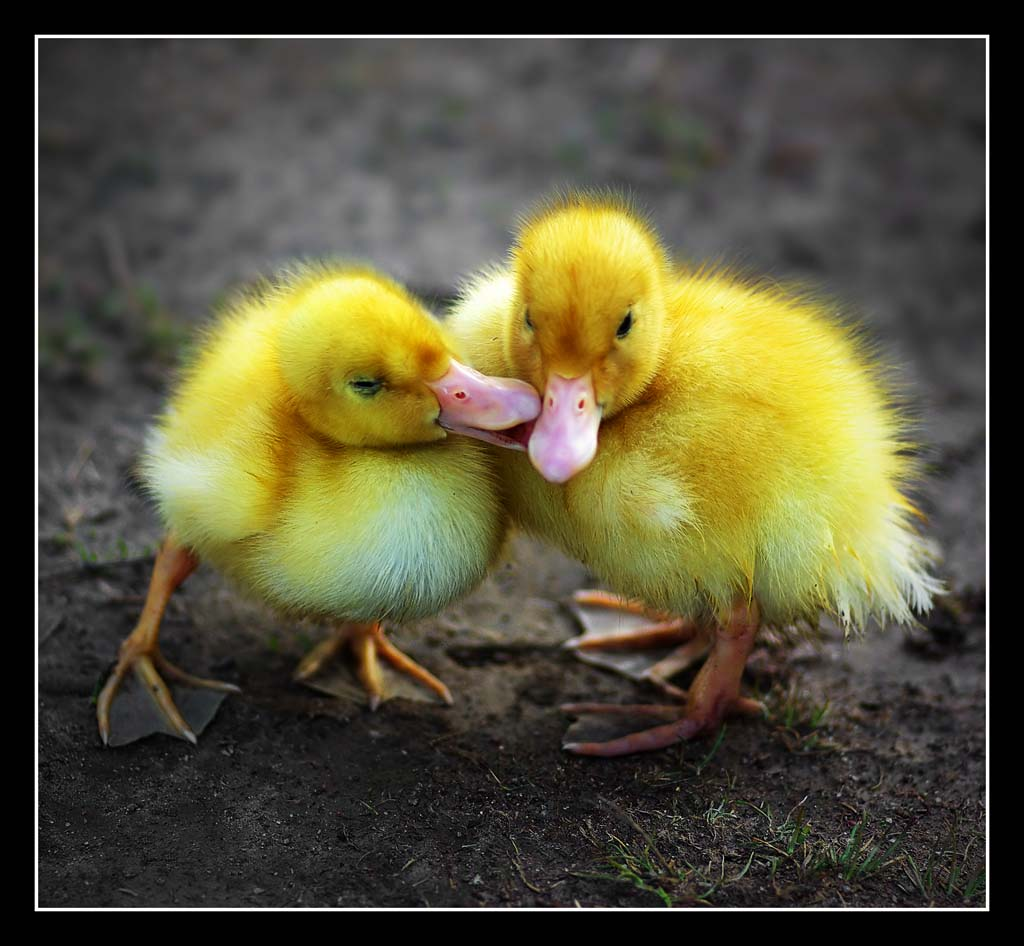
\includegraphics[height=\dimexpr11\textheight/16\relax]{ducks}
    \caption{Kissing ducks}
  \end{figure}
\end{frame}


\begin{frame}
  {A Movie}

  \begin{block}
    {Some block}

    \begin{itemize}
    \item Movies only seem to work in Adobe Reader
    \item Movie file is not embedded, it must be on the computer
    \end{itemize}
  \end{block}

  \pause
  \begin{alertblock}
    {Some more block}

    Movies only seem to work in Adobe Reader\par
    Movie file is not embedded, it must be on the computer
  \end{alertblock}
  \pause

  \begin{exampleblock}{}
    Some text in here.

    \begin{itemize}[<+->]
    \item Movies only seem to work in Adobe Reader
    \item Movie file is not embedded, it must be on the computer and
      what happe with a very long item?
    \end{itemize}
  \end{exampleblock}
\end{frame}


\section
  {Conclusion}

\begin{bibunit}[plain]
\begin{frame}
  {Credits}

  \begin{itemize}
  \item Brought to you by Cédric Mauclair
  \item Please let me know about improvements!
  \item Inspiration: \url{http://www.shawnlankton.com}... (in code)
  \end{itemize}

  \nocite{ipsum}
  \bibliography{demo}

\end{frame}
\end{bibunit}

\begin{bibunit}[plain]
\begin{frame}
  {Questions}

  \nocite{lorem}
  \bibliography{demo}

\end{frame}
\end{bibunit}


\appendix[Appendices]

\begin{frame}
  \frametitle{First appendix}
\end{frame}

\begin{frame}
  \frametitle{Second appendix}
\end{frame}

\end{document}


%%% Local Variables:
%%% mode: latex
%%% TeX-master: "demo-slides.tex"
%%% End:
